% 第4章第3节：子集累计与 Möbius 反演（子集格与累计；Möbius 反演；反演的计算与算例；有限偏序集上的推广）。

\section{子集累计与 Möbius 反演}
\label{sec:comb-cumulative-inversion}

本节转向另一类问题。设想每个课程组合有一个总得分：单门课各有自己的贡献，某两门课同时选又会产生额外的配合效果，配合也可能是负的。我们能观察到的是每个组合的总得分，想知道的却是每个组合\emph{自身}贡献了多少。第~\ref{sec:comb-overlap-counting}节的容斥原理由各交集的大小恢复并集的大小，这里要做的是同一类“由累计量恢复局部量”的事，只是对象换成了一般的数值。本节只用有限求和与包含关系，不依赖上一节的单调或次模假设，也不是后面选择算法的前提。

\subsection{子集格与累计}
\label{sec:graph-setfn-subset-lattice}

累计沿包含关系进行，所以先把包含关系画出来。第~\ref{sec:prelim-order-relations}节已经说明，包含关系是幂集上的偏序。有限集合$V$的全部子集连同包含关系称为$V$的\term{子集格}（subset lattice）：两个子集的交是它们最大的公共子集，并是包含两者的最小集合。图~\ref{fig:comb-mobius-cumulative-local}按元素个数自下而上分层画出$V_0=\{1,2,3,4\}$的子集格，每条连线连接只差一个元素的两个子集，沿连线向上一步就是加入一个元素。图~\ref{fig:graph-setfn-subset-binary-cube}中的立方体正是三元底集的子集格。

从$S$出发沿连线一路向下能到达的子集，恰好是$S$的全部子集。例如从$\{1,3\}$向下只能到达$\{1\}$、$\{3\}$和空集。下面定义的累计值，正是沿这些向下的路径收集贡献。

\begin{figure}[!htb]
  \centering
  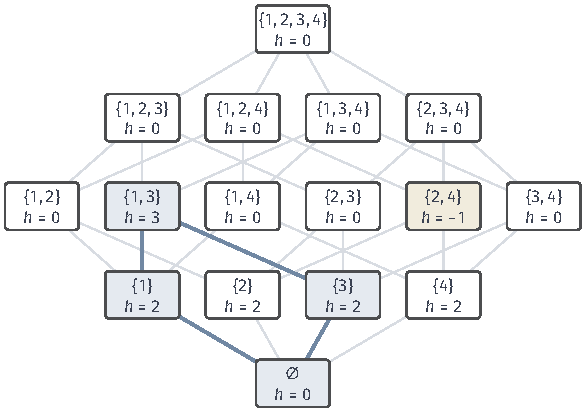
\includegraphics[width=99.187mm]{figures/01-basic-mathematics/04-graphs/tikz/c4-subset-lattice-cumulative/figure.pdf}
  \caption{四元素集合$V_0=\{1,2,3,4\}$的子集格与各子集自身的贡献$h$。子集按元素个数自下而上分层，连线连接只差一个元素的两个子集；框内上行为子集，下行为教学设定的贡献。蓝色标出$\{1,3\}$及其全部子集，它们的贡献相加得到累计值$g(\{1,3\})=0+2+2+3=7$；黄色框$\{2,4\}$的自身贡献为负。}
  \label{fig:comb-mobius-cumulative-local}
\end{figure}

\paragraph{自身贡献与累计值}
给每个子集$T$指定一个实数$h(T)$，表示$T$作为整体\emph{自身}带来的贡献：单元素集的贡献是单门课的得分，二元集的贡献是两门课的配合效果，依此类推。$S$的累计值收集它的全部子集的贡献：
\begin{equation}
  g(S)=\sum_{T\subseteq S}h(T).
  \label{eq:comb-zeta-transform}
\end{equation}
$g$与$h$都是$V$上的集合函数。注意累计不只相加单元素的贡献，$S$内部更大子集的配合贡献也计入其中。

图~\ref{fig:comb-mobius-cumulative-local}的教学设定让四个单项各贡献$2$，$\{1,3\}$另有配合贡献$3$，$\{2,4\}$另有配合贡献$-1$，其余子集（包括空集和全部三元、四元子集）的贡献为$0$。于是
\[
  g(\{1,3\})=h(\varnothing)+h(\{1\})+h(\{3\})+h(\{1,3\})=0+2+2+3=7,
\]
而两个单项的累计值之和只有$g(\{1\})+g(\{3\})=4$，多出的$3$正是$\{1,3\}$自身的贡献。反演要回答相反方向的问题：只知道每个子集的累计值$g$，怎样读出每个子集自身的贡献$h$。

\subsection{Möbius 反演}
\label{sec:graph-setfn-mobius-inversion}

先看两元素的情形。$g(\{1,3\})$包含$h(\varnothing)$、$h(\{1\})$、$h(\{3\})$和$h(\{1,3\})$四项。减去$g(\{1\})=h(\varnothing)+h(\{1\})$和$g(\{3\})=h(\varnothing)+h(\{3\})$，两个单项贡献被去掉，但$h(\varnothing)$被多减了一次，再加回$g(\varnothing)=h(\varnothing)$，剩下的恰是
\[
  h(\{1,3\})=g(\{1,3\})-g(\{1\})-g(\{3\})+g(\varnothing).
\]
符号按子集比$S$少几个元素交替变化。一般情形的公式正是这样，称为\term{Möbius反演}（Möbius inversion）。

\begin{theorem}[子集格上的 Möbius 反演]
\label{thm:comb-mobius-inversion}
设$V$为有限集合，$g,h:\mathcal P(V)\to\mathbb R$。若对每个$S\subseteq V$式~\eqref{eq:comb-zeta-transform}成立，则对每个$S\subseteq V$有
\begin{equation}
  h(S)=\sum_{T\subseteq S}(-1)^{|S|-|T|}g(T).
  \label{eq:comb-mobius-inversion}
\end{equation}
反过来，若对每个$S$式~\eqref{eq:comb-mobius-inversion}成立，则式~\eqref{eq:comb-zeta-transform}也对每个$S$成立。
\end{theorem}

\begin{proof}
把式~\eqref{eq:comb-zeta-transform}代入式~\eqref{eq:comb-mobius-inversion}右侧，得到对全部满足$R\subseteq T\subseteq S$的集合对$(R,T)$的双重和。先固定$T$再取$R$，与先固定$R$再取$T$，遍历的是同一批集合对，所以可以像第~\ref{sec:prelim-finite-sums-products}节的三角形求和那样交换有限求和的次序：
\[
  \sum_{T\subseteq S}(-1)^{|S|-|T|}\sum_{R\subseteq T}h(R)
  =\sum_{R\subseteq S}h(R)\sum_{T:\,R\subseteq T\subseteq S}(-1)^{|S|-|T|}.
\]
固定$R$后，满足$R\subseteq T\subseteq S$的$T$由$S\setminus R$中哪些元素被加入决定，即$T=R\cup D$，$D\subseteq S\setminus R$任意，且$|S|-|T|=|S\setminus R|-|D|$。记$q=|S\setminus R|$，按$|D|=j$分组，大小为$j$的$D$有$\binom qj$个，所以内层和等于
\[
  \sum_{j=0}^{q}\binom qj(-1)^{q-j}=(-1)^q\sum_{j=0}^{q}(-1)^j\binom qj
  =\begin{cases}1,&q=0,\\0,&q\geq1,\end{cases}
\]
最后一步用式~\eqref{eq:comb-alternating-subset-count}。内层和只在$R=S$时为$1$，在$R$是$S$的真子集时为$0$，所以真子集上的贡献全部抵消，右侧只剩$h(S)$。

反方向同样直接核对。由式~\eqref{eq:comb-mobius-inversion}给出$h$，代入$\sum_{T\subseteq S}h(T)$并交换求和次序，
\[
  \sum_{T\subseteq S}h(T)=\sum_{R\subseteq S}g(R)\sum_{T:\,R\subseteq T\subseteq S}(-1)^{|T|-|R|}.
\]
仍写$T=R\cup D$，内层和等于$\sum_{j=0}^{q}(-1)^j\binom qj$，它在$R=S$时只有$D=\varnothing$一项而等于$1$，在$R\neq S$时为$0$。所以右侧等于$g(S)$。
\end{proof}

定理说明式~\eqref{eq:comb-zeta-transform}与式~\eqref{eq:comb-mobius-inversion}是一对互逆的变换：从贡献到累计，再从累计回到贡献，不丢失任何信息。证明中起作用的是组合数的交错和为零，这与容斥原理的证明相同。区别在于，容斥最终使并集中的每个元素恰计一次，反演最终只保留指定子集自身的贡献。

\subsection{反演的计算与算例}
\label{sec:graph-setfn-mobius-computation}

\paragraph{四元素算例}
记$\mathbb I\{\cdot\}$为条件成立时取$1$、否则取$0$的指示函数。沿用图~\ref{fig:comb-mobius-cumulative-local}的设定，累计值可以写成
\[
  g(S)=2|S|+3\,\mathbb I\{\{1,3\}\subseteq S\}-\mathbb I\{\{2,4\}\subseteq S\}.
\]
其中$2|S|$收集$S$中各单项的贡献，后两项在$S$包含$\{1,3\}$或$\{2,4\}$时计入相应的配合贡献。表~\ref{tab:comb-four-element-mobius}列出全部$16$个累计值，以及只用这些累计值按式~\eqref{eq:comb-mobius-inversion}恢复的贡献。

\begin{table}[!htb]
  \centering
  \begin{tabular}{ccc@{\qquad}ccc}
    \toprule
    $S$ & $g(S)$ & $h(S)$ & $S$ & $g(S)$ & $h(S)$ \\
    \midrule
    $\varnothing$ & $0$ & $0$ & $\{2,3\}$ & $4$ & $0$ \\
    $\{1\}$ & $2$ & $2$ & $\{2,4\}$ & $3$ & $-1$ \\
    $\{2\}$ & $2$ & $2$ & $\{3,4\}$ & $4$ & $0$ \\
    $\{3\}$ & $2$ & $2$ & $\{1,2,3\}$ & $9$ & $0$ \\
    $\{4\}$ & $2$ & $2$ & $\{1,2,4\}$ & $5$ & $0$ \\
    $\{1,2\}$ & $4$ & $0$ & $\{1,3,4\}$ & $9$ & $0$ \\
    $\{1,3\}$ & $7$ & $3$ & $\{2,3,4\}$ & $5$ & $0$ \\
    $\{1,4\}$ & $4$ & $0$ & $V_0$ & $10$ & $0$ \\
    \bottomrule
  \end{tabular}
  \caption{四元素子集格上的累计值$g$与由式~\eqref{eq:comb-mobius-inversion}恢复的自身贡献$h$。恢复结果与教学设定一致：四个单项各为$2$，$\{1,3\}$为$3$，$\{2,4\}$为$-1$，其余子集（包括全部三元子集和$V_0$）均为$0$。}
  \label{tab:comb-four-element-mobius}
\end{table}

两个二元子集的贡献按上一小节的四项公式恢复：
\[
  h(\{1,3\})=7-2-2+0=3,\qquad h(\{2,4\})=3-2-2+0=-1.
\]
三元子集要用到八个累计值。对$S=\{1,2,3\}$，按子集大小依次取三元、二元、一元和空集项，
\[
  h(\{1,2,3\})=9-(4+7+4)+(2+2+2)-0=0.
\]
虽然$\{1,2,3\}$包含有配合效果的$\{1,3\}$，它的累计值$9$也大于三个单项之和$6$，但多出的$3$已经由$h(\{1,3\})$解释，三门课之间没有新的整体效果，所以三元贡献为$0$。$\{1,3,4\}$也是如此：$g=9$，恢复出$h=0$。反演还允许贡献为负，$h(\{2,4\})=-1$就是一例。

\paragraph{按子集大小递推}
式~\eqref{eq:comb-mobius-inversion}给出每个$h(S)$的显式公式。另一种做法直接由式~\eqref{eq:comb-zeta-transform}移项：
\[
  h(S)=g(S)-\sum_{T\subsetneq S}h(T).
\]
输入是全部$2^n$个累计值；从$h(\varnothing)=g(\varnothing)$出发，按元素个数从小到大计算，算到$S$时它的全部真子集的$h$都已求出；输出是全部$2^n$个贡献。在上面的算例中，先得到空集和四个单项，再由$h(\{1,3\})=7-(0+2+2)=3$等算出二元贡献，最后算三元与四元贡献。

两种做法的开销相同。处理$S$时都要遍历它的$2^{|S|}$个子集，按大小分组求和，总次数为
\[
  \sum_{k=0}^{n}\binom nk2^k=3^n,
\]
最后一步是二项式定理。输入本身已有$2^n$个数，所以这里没有多项式规模的算法：单个递推式写起来简短，并不意味着整个问题便宜。

若要进一步减少运算，可以逐个元素做差分：对$i=1,\ldots,n$依次执行“对每个含$i$的$S$，把当前存储的值$g(S)$替换为$g(S)-g(S\setminus\{i\})$”（同一轮中用的都是上一轮的值）。对$i$归纳可以核对，处理完元素$1,\ldots,i$后，$S$处存储的值等于$\sum(-1)^{|S|-|T|}g(T)$，其中$T$取遍满足$T\subseteq S$且与$S$在元素$i+1,\ldots,n$上一致的子集；$i=n$时这正是式~\eqref{eq:comb-mobius-inversion}。每轮做$2^{n-1}$次减法，总共$n2^{n-1}$次，仍随$n$指数增长，只是比$3^n$小。

\subsection{有限偏序集上的推广}
\label{sec:graph-setfn-poset-mobius}

反演公式中的系数$(-1)^{|S|-|T|}$只依赖两个子集的相对位置。同样的问题可以在任意有限偏序集$(X,\preceq)$上提出：给每个元素$y$一个数$h(y)$，沿下方累计得$g(x)=\sum_{y\preceq x}h(y)$，再问怎样由$g$恢复$h$。这时系数不再一律是$\pm1$，而由下面的函数确定。

\begin{definition}[Möbius 函数]
\label{def:graph-setfn-mobius-function}
设$(X,\preceq)$是有限偏序集，记$y\prec x$表示$y\preceq x$且$y\neq x$。偏序集的\term{Möbius函数}（Möbius function）$\mu$对满足$y\preceq x$的元素对定义为
\[
  \mu(y,y)=1,\qquad \mu(y,x)=-\sum_{z:\,y\preceq z\prec x}\mu(y,z)\quad(y\prec x),
\]
对不满足$y\preceq x$的元素对取$\mu(y,x)=0$。
\end{definition}

定义固定区间的下端$y$，从对角值$\mu(y,y)=1$出发向上递推：区间$\{z:y\preceq z\preceq x\}$越长，需要的已知值越多，而有限偏序集保证递推在有限步内完成。递推式移项后写成
\[
  \sum_{z:\,y\preceq z\preceq x}\mu(y,z)=0\qquad(y\prec x),
\]
即每个非平凡区间上的系数之和为零。这正是反演证明中内层和所需的抵消，所以按与定理~\ref{thm:comb-mobius-inversion}相同的交换求和论证，可以得到$h(x)=\sum_{y\preceq x}\mu(y,x)g(y)$。

\paragraph{子集格的系数}
在子集格上取$\mu(T,S)=(-1)^{|S|-|T|}$。对$T\subsetneq S$，记$q=|S\setminus T|\geq1$，
\[
  \sum_{R:\,T\subseteq R\subseteq S}(-1)^{|R|-|T|}=\sum_{j=0}^{q}(-1)^j\binom qj=0,
\]
这正是上面的递推式。所以子集格上的反演系数只取$\pm1$，式~\eqref{eq:comb-mobius-inversion}是一般结构的特例。

\paragraph{整除偏序的例子}
图~\ref{fig:graph-setfn-mobius-divisors}是$12$的六个正因数在整除关系下的偏序。从$\mu(1,1)=1$出发，$\mu(1,2)=\mu(1,3)=-1$；区间$\{1,2,4\}$是一条链，$\mu(1,4)=-(1-1)=0$；区间$\{1,2,3,6\}$与两元素的子集格形状相同，$\mu(1,6)=-(1-1-1)=1$；最后$\mu(1,12)=-(1-1-1+0+1)=0$。系数出现了$0$，说明一般偏序上的反演确实不同于子集格上的交错加减。本小节只作为有限组合结构的补充，不涉及无限偏序和收敛问题，后面的选择算法也不以它为前提。

\begin{figure}[!htb]
  \centering
  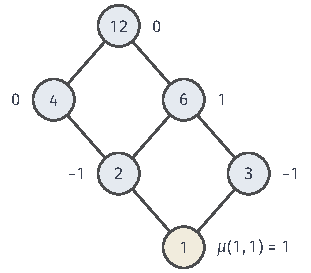
\includegraphics[width=52.613mm]{figures/01-basic-mathematics/04-graphs/tikz/c4-mobius-divisor-poset/figure.pdf}
  \caption{$12$的正因数在整除关系下的偏序，连线连接直接相邻的两个因数，下方整除上方。节点旁的数是$\mu(1,x)$，由$\mu(1,1)=1$（黄色节点）自下而上递推得到。链$1\mid2\mid4$上$\mu(1,4)=0$，与子集格同形的区间$\{1,2,3,6\}$上$\mu(1,6)=1$。}
  \label{fig:graph-setfn-mobius-divisors}
\end{figure}
